%\chapter{Lesson 18.03.2020} % 18 marzo 2020
\lesson{4}{18/03/2020}
\noindent Since we are interested in pricing simple options, we consider a \emph{stationary binomial recombining tree} or \emph{lattice}, i.e. a model in which the way the underlying goes up and down increases or decreases is always the same.

\section{Binomial lattice}
\subsection{Pricing options}
Consider the following binomial lattice:
\begin{center}
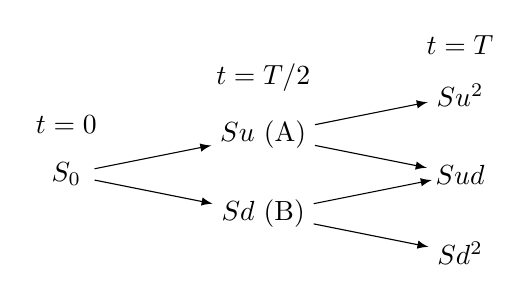
\begin{tikzpicture}[
                   grow = right,
edge from parent/.style = {draw,-latex},
         label distance = 1.5mm,
      every node/.style = {minimum width=2em, inner sep=3pt},
         level distance = 25mm,
       sibling distance = 10mm,
                     ]
\node[label=90:{$t=0$}] {$S_0$}
    child {node {$Sd$ (B)}
        child {node {$Sd^2$}
            %child {node {40}}
            %child {node {20}}
                }
        child {node {}}%<---------------- already printed
            }
    child {node[label=90:{$t=T/2$}] {$Su$ (A)}
        child {node {$Sud$}
            %child {node {}}%<------------ already printed
            %child {node {0}}
                }
        child {node[label=90:{$t=T$}] {$Su^2$}
            %child {node {}}%<------------ already printed
            %child {node[label=90:{$t=3$}] {0}}
                }
                };
\end{tikzpicture}
\end{center}
and a call option, whose payoff is the random vector
\begin{equation*}
    \mbox{payoff}_T = \left(
    \begin{matrix}
        (Su^2-K)^+ \\ (Sud-K)^+ \\ (Sd^2-K)^+
    \end{matrix}
    \right) 
    =
    \left(
    \begin{matrix}
        f^{u^2} \\ f^{ud} \\ f^{d^2}
    \end{matrix}
    \right) 
\end{equation*}
The problem is always the same: how much do we have to pay at time $t=0$ in order to get this payoff at time $t=T$?\\
Suppose that we are in node (A). According to the risk neutral methodology, the value of the relative sub-payoff is given by
\begin{align}
    \notag Value_A\left(\binom{f^{u^2}}{f^{ud}}\right) 
    &= 
    \notag e^{-R\frac{T}{2}}\mathbb{E}^{\Qmeas}\left(\left.\binom{f^{u^2}}{f^{ud}}\right|\mbox{(A)}\right)\\
    &=
    e^{-R\frac{T}{2}}(qf^{u^2}+(1-q)f^{ud})
\end{align}
where
\begin{equation}\label{qT2}
    q = \dfrac{e^{R\frac{T}{2}}-d}{u-d}
\end{equation}
Notice that in this case the expected value is a conditional expected value. In analogy, in the node (B) we have
\begin{equation}
    Value_B\left(\binom{f^{ud}}{f^{d^2}}\right) = e^{-R\frac{T}{2}}(qf^{ud}+(1-q)f^{d^2})
\end{equation}
Now, we can compute the initial price of the whole payoff:
\begin{align}
    \notag price_0\left(
    \begin{matrix}
        f^{u^2} \\ f^{ud} \\ f^{d^2}
    \end{matrix}
    \right) 
    &= 
    price_0\left(\begin{matrix}
        Value_A \\  Value_B
    \end{matrix}\right)\\
    %\binom{Value_{(A)}}{Value_{(B)}} \\
    &=
    \notag e^{-R\frac{T}{2}}\mathbb{E}^{\Qmeas}\left[\left(
    \begin{matrix}
        Value_A \\  Value_B
    \end{matrix}\right)
    %\binom{Value_{(A)}}{Value_{(B)}}
    \right]\\
    &=
    \notag e^{-R\frac{T}{2}}(q Value_A+(1-q)Value_B)\\
    &=
    \notag e^{-R\frac{T}{2}}\left[q\left(e^{-R\frac{T}{2}}(qf^{u^2}+(1-q)f^{ud})\right) + (1-q)\left(e^{-R\frac{T}{2}}(qf^{ud}+(1-q)f^{d^2})\right)\right]\\
    &=
    e^{-RT}[q^2f^{u^2}+2q(1-q)f^{ud}+(1-q)f^{d^2}]
\end{align}
Notice that the three coefficients are positive and their sum gives 1, so again we obtained a convex combination of elements, i.e. an expected value:
\begin{equation}
    price_0
    \left(
    \begin{matrix}
        f^{u^2} \\ f^{ud} \\ f^{d^2}
    \end{matrix}
    \right) 
    = e^{-RT} \mathbb{E}^{\Qmeas}
    \left[ 
    \left(
    \begin{matrix}
        f^{u^2} \\ f^{ud} \\ f^{d^2}
    \end{matrix}
    \right)
    \right] 
    = e^{-RT}\mathbb{E}^{\Qmeas}[\mbox{payoff}_T]
\end{equation}
The formula has the same form as before but it must be contextualized as the expectation under the risk neutral probability measure 
\begin{equation}
    Q \sim 
    \left(
    \begin{matrix}
        q \\ 2q(1-q) \\ q^2
    \end{matrix}
    \right)
\end{equation}

\subsection{Hedging}
We now want to implement the corresponding hedging portfolio, i.e. the replicating portfolio which allows the short position to construct the payoff for the long position. \\
First we have to solve the pricing procedure for all the intermediate nodes, in fact hedging is a forward procedure. Then, the number of shares we have to put in our portfolio is
\begin{equation}
    \Delta_0 = \dfrac{Value_A-Value_B}{Su-Sd}
\end{equation}
and the corresponding investment in the riskless market is
\begin{equation}
    \beta_0 = p_0-\Delta_0S
\end{equation}
where $p_0 = V_0 = price_0$. This is the initial step. Now we have to consider the intermediate step, according to the possible values of the underlying:
\begin{equation}
    \Delta_A = \dfrac{f^{u^2}-f^{ud}}{Su^2-Sud}, \qquad \Delta_B = \dfrac{f^{ud}-f^{d^2}}{Sud-Sd^2}
\end{equation}
Now we have
\begin{equation*}
    Value_A = \Delta_ASu+\beta_Ae^{R\frac{T}{2}}, \qquad Value_B = \Delta_BSd+\beta_Be^{R\frac{T}{2}}
\end{equation*}
so the investment in the riskless market is
\begin{equation}
    \beta_A = (Value_A-\Delta_ASu)e^{-R\frac{T}{2}}, \qquad \beta_B = (Value_B-\Delta_BSd)e^{R\frac{T}{2}}
\end{equation}
So, in a dynamic binomial model, also the hedging is dynamic. This is obvious, since we can exploit the possibility to change our strategy according to the fluctuations of the underlying.

\subsection{Dynamic interest rates}
\begin{remark}
There are two possible riskless assets: 
\begin{itemize}
    \item the one which consider the forward evolution of the asset, used for example in savings accounts
    \item the zero coupon bond, which consider the backward evolution of the asset
\end{itemize}
If the interest rate is constant, the two are equivalent. Moreover, the two are equivalent even if the interest rate evolves and its dynamic is deterministic.
\end{remark}
\noindent If we consider different maturity times we can find which is the corresponding value of one unit of cash, i.e. \EUR{1}. It is intuitive to expect that for a larger maturity there will be a larger interest rate. However, there are some cases in which the interest rate decreases in time. This typically happens after a financial crisis. In other cases the curve will assume other shapes, like the one in Figure \colorbox{magenta}{fig7}, which is typically used for large maturities, e.g. 30 years.
\begin{center}
    \colorbox{green}{fig7}
\end{center}
The input to find which is the interest rate corresponding to a certain maturity are the prices of the zero coupon bound. So, starting from now we have to take into account different rates with respect to different maturities. \\
Recall the binomial lattice
\begin{center}
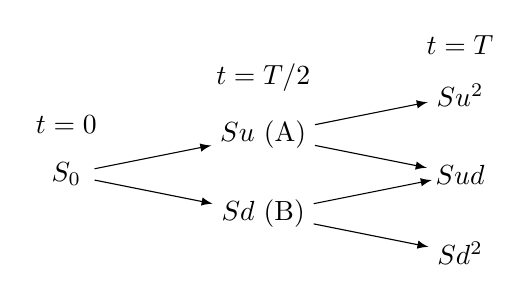
\begin{tikzpicture}[
                   grow = right,
edge from parent/.style = {draw,-latex},
         label distance = 1.5mm,
      every node/.style = {minimum width=2em, inner sep=3pt},
         level distance = 25mm,
       sibling distance = 10mm,
                     ]
\node[label=90:{$t=0$}] {$S_0$}
    child {node {$Sd$ (B)}
        child {node {$Sd^2$}
            %child {node {40}}
            %child {node {20}}
                }
        child {node {}}%<---------------- already printed
            }
    child {node[label=90:{$t=T/2$}] {$Su$ (A)}
        child {node {$Sud$}
            %child {node {}}%<------------ already printed
            %child {node {0}}
                }
        child {node[label=90:{$t=T$}] {$Su^2$}
            %child {node {}}%<------------ already printed
            %child {node[label=90:{$t=3$}] {0}}
                }
                };
\end{tikzpicture}
\end{center}
and focus on node (A). We have two different interest rates, $R_{\nicefrac{T}{2}}=R(0,\nicefrac{T}{2})$ and $R_T=R(0,T)$, called \emph{spot interest rates} because they start from $t=0$. The problem is to compute $q$: we would like to find an expression similar to \eqref{qT2} but we need $R=R(0,\nicefrac{T}{2},T)$ -- i.e. the interest rate decided at $t=0$ that starts to capitalize at $t=\nicefrac{T}{2}$ until $t=T$ -- which is not defined yet. $R=R(0,\nicefrac{T}{2},T)$ is called \emph{forward interest rate}. We would like to deduce the value of the forward interest rate starting from the spot interest rates. If we put \EUR{1} at $t=0$ we have 
\begin{equation*}
    1 \longrightarrow e^{R\left(0,\frac{T}{2}\right)\frac{T}{2}} \longrightarrow e^{R\left(0,\frac{T}{2}\right)\frac{T}{2}}e^{R\left(0,\frac{T}{2},T\right)\frac{T}{2}}
\end{equation*}
which has to be consistent with the one shot capitalization using
\begin{equation*}
    1\longrightarrow e^{R(0,T)T}
\end{equation*}
otherwise there is an arbitrage opportunity. We obtain the following equation:
\begin{equation}\label{equality}
    e^{R\left(0,\frac{T}{2}\right)\frac{T}{2}}e^{R\left(0,\frac{T}{2},T\right)\frac{T}{2}} = e^{R(0,T)T}
\end{equation}
which has solution
\begin{equation}
    R\left(0,\frac{T}{2},T\right) = \dfrac{R(0,T)T + R\left(0,\frac{T}{2}\right)\frac{T}{2}}{\frac{T}{2}}
\end{equation}
Now we can define the risk neutral probability in the node (A):
\begin{equation}
    q_A = \dfrac{e^{R\left(0,\frac{T}{2},T\right)\frac{T}{2}}-d}{u-d} 
\end{equation}
The same argument holds for node (B), so the expression for $q_B$ is exactly the same of $q_A$. The interest rate at $t=0$ will be
\begin{equation}
    q_0 = \dfrac{e^{R\left(0,\frac{T}{2}\right)\frac{T}{2}}-d}{u-d} 
\end{equation}
So, denoting $q_A = q_B \equiv q_1$, the price at $t=0$ is given by
\begin{equation}\label{p00}
    price_0
    \left(
    \begin{matrix}
        f^{u^2} \\ f^{ud} \\ f^{d^2}
    \end{matrix}
    \right) 
    = e^{-R(0,T)T} \mathbb{E}^{\Qmeas}[\mbox{payoff}_T]
\end{equation}
where
\begin{equation}
    Q \sim \left(
    \begin{matrix}
        q_0q_1 \\ q_0(1-q_1)+(1-q_0)q_1 \\ (1-q_0)(1-q_1)
    \end{matrix}
    \right) 
\end{equation}
Expanding \eqref{p00} we get 
\begin{equation}
    price_0
    \left(
    \begin{matrix}
        f^{u^2} \\ f^{ud} \\ f^{d^2}
    \end{matrix}
    \right) 
    = e^{-R(0,T)T}(f^{u^2}q_0q_1 + f^{ud}(q_0(1-q_1)+(1-q_0)q_1) + f^{d^2}(1-q_0)(1-q_1))
\end{equation}